% The three R-hadron sectors in the static-gluino limit, as lattice correlators.
% Time runs upward.  The gluino is an adjoint Wilson line (double gold line) at a fixed site;
% operators of the light degrees of freedom sit at its ends.
\documentclass[tikz,border=6pt]{standalone}
\usepackage{amsmath,amssymb}
\usetikzlibrary{decorations.pathmorphing,decorations.markings,arrows.meta,calc,patterns,shapes.geometric}
\definecolor{ink}{HTML}{222222}
\definecolor{gold}{HTML}{C8961E}
\definecolor{acc}{HTML}{B2182B}
\definecolor{blu}{HTML}{2166AC}
\definecolor{grn}{HTML}{4D9221}
\definecolor{lat}{HTML}{C9C9C9}
\tikzset{
  adj/.style={double=gold!80, double distance=1.6pt, draw=gold!60!black, line width=0.5pt},
  op/.style={fill=white, draw=ink, line width=0.6pt, minimum size=5pt, inner sep=0pt},
  quark/.style={line width=0.9pt, draw=#1, postaction={decorate}, decoration={markings,
     mark=at position 0.55 with {\arrow{Stealth[length=4pt]}}}},
  glue/.style={draw=acc, line width=0.8pt, decorate, decoration={coil, aspect=0.6, segment length=3.2pt, amplitude=1.6pt}},
  lab/.style={font=\small, text=ink},
  small/.style={font=\scriptsize, text=ink!70},
}
% one spacetime slab: x horizontal, t vertical, a little perspective in the depth direction
\newcommand{\slab}{%
  \foreach \t in {0,...,6} \draw[lat, line width=0.3pt] (-1.6,\t*0.55) -- (1.6,\t*0.55);
  \foreach \x in {-1.6,-0.8,0,0.8,1.6} \draw[lat, line width=0.3pt] (\x,0) -- (\x,3.3);
  \foreach \x in {-1.6,-0.8,0,0.8,1.6} \foreach \t in {0,...,6} \fill[lat] (\x,\t*0.55) circle (0.6pt);
}
\begin{document}
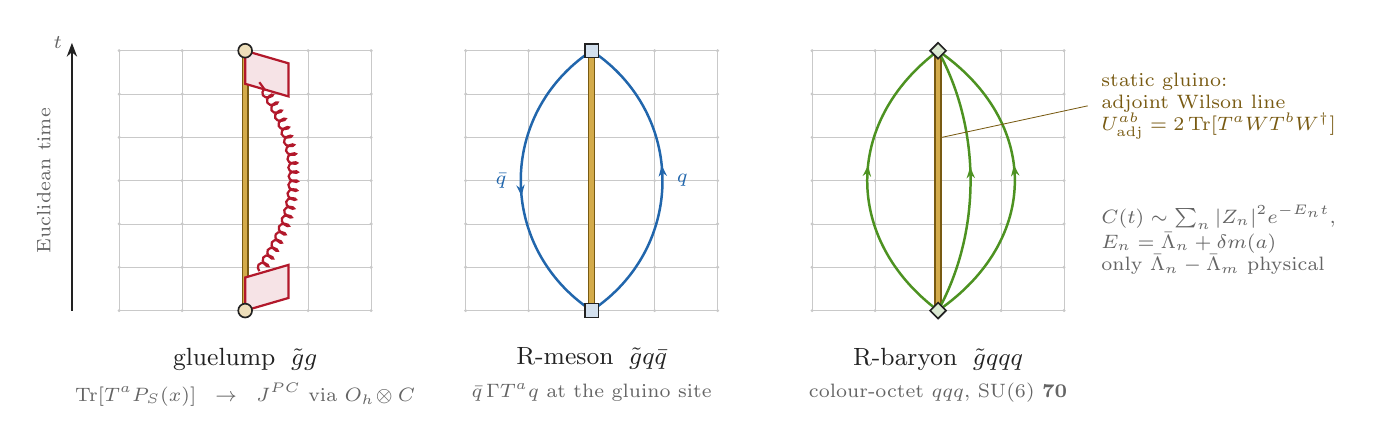
\begin{tikzpicture}[x=1cm,y=1cm]
  % ---------------- gluelump --------------------------------------------------------------
  \begin{scope}[shift={(0,0)}]
    \slab
    \draw[adj] (0,0) -- (0,3.3);
    % spatial loop operators at source and sink (traceless octet part of a closed path)
    \foreach \t/\d in {0/1, 3.3/-1} {
      \draw[acc, line width=0.8pt, fill=acc!12] (0,\t) -- ++(0.55,0.16*\d) -- ++(0,0.42*\d) -- ++(-0.55,-0.16*\d) -- cycle;
      \node[op, circle, fill=gold!30] at (0,\t) {};
    }
    \draw[glue] (0.18,0.5) .. controls (0.75,1.3) and (0.75,2.1) .. (0.18,2.9);
    \node[lab, anchor=north] at (0,-0.35) {gluelump\; $\tilde g g$};
    \node[small, anchor=north] at (0,-0.8) {$\operatorname{Tr}[T^a P_S(x)]\;\;\to\;\;J^{PC}$ via $O_h\!\otimes C$};
  \end{scope}
  % ---------------- R-meson ---------------------------------------------------------------
  \begin{scope}[shift={(4.4,0)}]
    \slab
    \draw[adj] (0,0) -- (0,3.3);
    \draw[quark=blu] (0,0) .. controls (1.2,0.8) and (1.2,2.5) .. (0,3.3);
    \draw[quark=blu] (0,3.3) .. controls (-1.2,2.5) and (-1.2,0.8) .. (0,0);
    \node[op, rectangle, fill=blu!20] at (0,0) {};
    \node[op, rectangle, fill=blu!20] at (0,3.3) {};
    \node[small, text=blu] at (1.15,1.65) {$q$};
    \node[small, text=blu] at (-1.15,1.65) {$\bar q$};
    \node[lab, anchor=north] at (0,-0.35) {R-meson\; $\tilde g q\bar q$};
    \node[small, anchor=north] at (0,-0.8) {$\bar q\,\Gamma T^a q$ at the gluino site};
  \end{scope}
  % ---------------- R-baryon --------------------------------------------------------------
  \begin{scope}[shift={(8.8,0)}]
    \slab
    \draw[adj] (0,0) -- (0,3.3);
    \draw[quark=grn] (0,0) .. controls (1.3,0.9) and (1.3,2.4) .. (0,3.3);
    \draw[quark=grn] (0,0) .. controls (0.55,1.0) and (0.55,2.3) .. (0,3.3);
    \draw[quark=grn] (0,0) .. controls (-1.2,0.9) and (-1.2,2.4) .. (0,3.3);
    \node[op, diamond, fill=grn!20, minimum size=6pt] at (0,0) {};
    \node[op, diamond, fill=grn!20, minimum size=6pt] at (0,3.3) {};
    \node[lab, anchor=north] at (0,-0.35) {R-baryon\; $\tilde g qqq$};
    \node[small, anchor=north] at (0,-0.8) {colour-octet $qqq$, SU(6) $\mathbf{70}$};
  \end{scope}
  % ---------------- shared annotations -----------------------------------------------------
  \draw[-{Stealth[length=5pt]}, ink, line width=0.5pt] (-2.2,0) -- (-2.2,3.4) node[left, small] {$t$};
  \node[small, rotate=90, anchor=south] at (-2.35,1.65) {Euclidean time};
  \node[small, text=gold!60!black, anchor=west, align=left] at (10.75,2.6)
    {static gluino:\\adjoint Wilson line\\$U_{\rm adj}^{ab} = 2\operatorname{Tr}[T^a W T^b W^\dagger]$};
  \draw[gold!60!black, line width=0.3pt] (10.7,2.6) -- (8.85,2.2);
  \node[small, anchor=west, align=left] at (10.75,0.9)
    {$C(t)\sim \sum_n |Z_n|^2 e^{-E_n t}$,\\$E_n = \bar\Lambda_n + \delta m(a)$\\only $\bar\Lambda_n-\bar\Lambda_m$ physical};
\end{tikzpicture}
\end{document}
